\documentclass{article}
\usepackage[utf8]{inputenc}
\usepackage{graphicx}

\title{Nose and Smell}
\author{MCB C61 with Professor David Presti \\ \\ Benjamin Lee}
% \date{8 March 2018}

\begin{document}

\maketitle

\textbf{Key Concepts:}
\begin{itemize}
    \item olfaction
    \item olfactory recptor cells
    \item olfactory stem cells
    \item cilia
    \item olfactory receptor proteins
    \item psudogene
    \item essential oil
    \item aromas: mixtures of molecules vs single molecules
    \item spices as aromatics
    \item sulfur, thiols
    \item anosmia: specific and general
    \item olfactory bulb
    \item pheromones, vomeronasal organ
\end{itemize}

\newpage

\section{Olfactory Sensory Perception}

\textbf{Olfaction:} the action or capacity of smelling; the sense of smell \\
\textbf{Odorants:} airborne volatile molecules \\

Olfactory sensory perception begins when odorants enter the nasal passages. Some are caught in the moist and mucousy tissue lining the interior of the nasal passages, known as the \textbf{nasal or olfactory epithelium}. (\textit{Epithelium} is the name given to the types of cells that line the surfaces of many strutures throughout the body.)\\ 

\begin{figure}[htp]
\centering
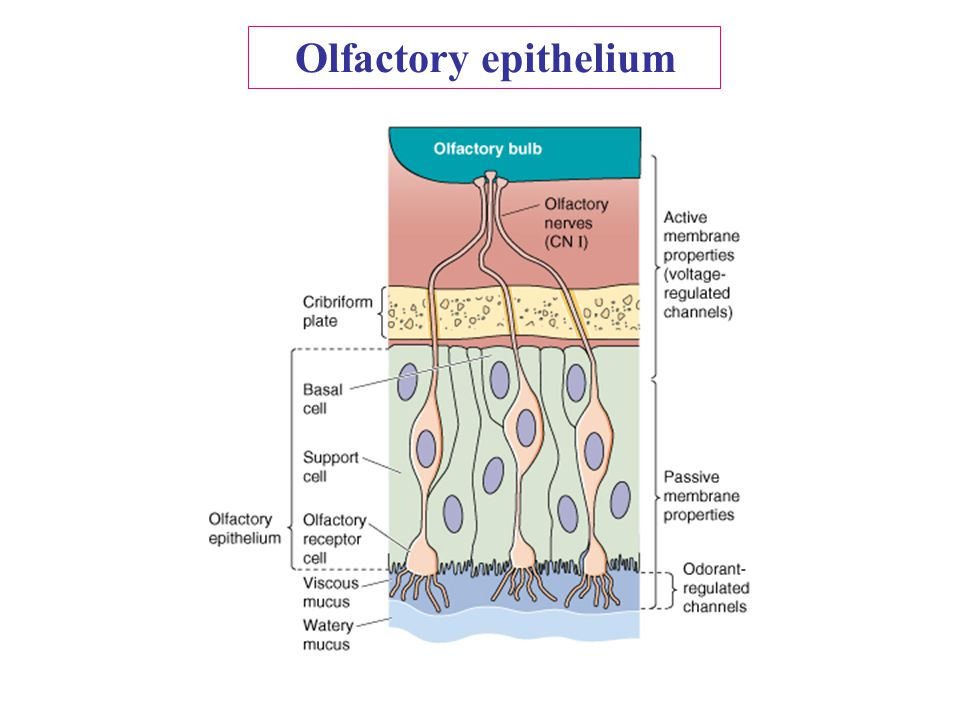
\includegraphics[width=13cm]{images/olfactoryepithelium.jpg}
\caption{Olfactory Epithelium}
\label{fig: OE}
\end{figure}

\textbf{Olfactory receptor cells} are embedded in the nasal epithelium. The dendrites of the receptor cells branch into \textbf{cilia} containing \textbf{olfactory receptor proteins}. The cilia extend into the \textbf{mucus lining} the nasal passage creating a large surface area containing olfactory receptor proteins. \\

\textbf{Olfactory stem cells} can only differentiate into various different types of olfactory receptor cells (unlike primordial stem cells that can differentiate into any kind of cell). This allows for the receptor cells to be regularly replaced (happens every month or two.). Beneficial because direct exposure of the receptor cells to potentially toxic substances, resulting in cellular damage (cost of chemoreception)\\

\subsection{Olfactory Receptor Proteins}
Olfactory receptors are \textbf{G-protein-coupled receptors} (GPCRs) \\
Number of different types of \textit{olfactory receptor proteins} varies widely by species. 
\begin{itemize}
    \item Fish have 100 different olfactory receptor proteins coded by 100 different genes
    \item Mammals have around 1,000 different olfactory receptor proteins
    \item Mice have about 13,000 different olfactory receptor proteins
    \item Humans have about 350 different olfactory receptor proteins
\end{itemize}
Each different GPCR responds to molecules having specific molecular shape. \\

\textbf{Pseudogenes:} nonfunctional genes that, although they appear to code for olfactory proteins, are altered in some way so that they do not code for functional receptor proteins. \\

\noindent Humans have about 600 olfactory pseudogenes. It is thought that our distant ancestors had many more functional olfactory receptor types, making our smell more sophisticated. But our evolutionary time line has made us stand upright and away from the ground, making us rely more on our eyes and less on our nose. \\

\noindent How can we still detect thousands of different odors with only 350 olfactory proteins? \\
An odor may bind to several different GPCRs all at varying levels of activation. So it becomes possible to discriminate large numbers of odorant molecules. \\

\newpage
\section{Essential Oils, Aromas, and Spices}

\textbf{Essential oil} designates the oily concentrate of aromatic molecules from a plant. \textit{Essential} (esse = to be) refers to the distinctive scent of the plant, its hallmark aroma. It is oily because the aroma-carrying molecules frequently are hydrophobic.\\

\textbf{Aroma and aromatic} derive from the Greek word for spice. Spices are key to aromatic substances and have been highly valued due to the olfactory qualities they add to food and perfumes. \\

\noindent Examples: \textbf{Mixture molecules vs. Single molecules} \\
(Main point of chemicals is to note how many different chemicals react with our olfactory receptor GPCRs to produce a wonderful mental experience of aroma)\\
\begin{itemize}
    \item Cinnamon (Cinnamomum verum)
        \subitem Native to Southeast Asia region
        \subitem The bark of these plant species contains highly aromatic essential oil, used in both savory and sweet foods
        \subitem Essential oil contains a complex mixture of chemical components: cinnamaldehyde, cinnamyl acetate, cinnamyl alcohol, copaene, eugenol, ethyl cinnamate, guaiene, and more
        \subitem We smell all of these molecules with our 350 types of olfactory receptor GPCRs in our nasal eipthelium to get the aroma that is cinnamon
    \item Cardamom (Elettaria cardamomum)
        \subitem Seeds used to flavor Indian foods, tea and coffee. 
        \subitem \textit{Aromatic essence} contains dozens of molecules: limonene, menthone, euxalyptol, terpineol, terpenylacetate, myrcene, sabinene, phellandrene, etc. 
    \item Black Pepper (Piper nigrum)
        \subitem Native to India
        \subitem \textit{Aromatic essence} a mixture of numerous molecules: sabinene, linalool, piperine, limonene, caryophyllene, pinene, carene, etc.
    \item Roses (genus \textit{Rosa})
        \subitem Many variants having flowers of different shapes, sizes, colors, and aromas. 
        \subitem Chemical components of rose aroma: citronellol, geraniol, nerol, linalool, citral, and phenyl ethanol. 
        \subitem Citronellol, geraniol, and nerol have similar molecular shapes. Roses smell differently because they have different relative amounts of these and other molecules that make up there aromatic essential oil. 
    \item Jasmine (genus \textit{Jasminum})
        \subitem Floral aroma derives from a mixture of molecules: benzyl acetate, indole, and farnesene. 
        \subitem Indole's aromatic quality is sharp and noxious, reminiscent of mothballs and feces. Although nasty, it is an alluring aroma of jasmine and is synergistic combination with dozens of other molecules. 
\end{itemize}

Although aromas consist of a complex arrangement of molecules, \textbf{often one or two molecules} in the mix identify strongly with the odor of the plant. \\

Such as benzyl acetate, which one could identify it with a jasmine aroma. \textit{Geranial} is a component of the essential oil of lemon. \textit{Geraniol} is a component of the essential oil of rose. Both when smelt are associated with its characteristic aroma. \\
Note geranial and geroniol differ by a double bound to an oxygen in geranial, but this subtle difference is enough to distinguish the associated aroma (lemon vs rose). (Idea: small molecule changes have profound changes in the way we perceive a smell) \\

\textbf{Natural vs Synthetic Aroma Products:} Most perfume products use synthetic molecules because obtaining the materials from the plants and animals is much more difficult. But this effort to mimic these aromas results in the loss of nuance from the original aromas. We can see this by the above molecules. Essential oils was the old way. \\

\subsection{Sulfur and Thiols}

These three molecules contain \textbf{sulfur-hydrogen (-SH)} groups. \\
\textit{Thio} refers to the element sulfur and \textit{Thiol} to the -SH group. 

\begin{itemize}
    \item 2-butene-1-thiol
    \item 3-methyl-1-butanethiol
    \item 2-quinolinemethanethiol
\end{itemize}

Examples of organic thiols, the -SH group is analogous to -OH groups in alcohol. The shape of -SH groups attached to carbons promotes fitting into GPCR olfactory receptors, which gives rise to a \textbf{stinky} smell reaction. Major chemical constituents of stinky secretions by skunks. \\

\textbf{Methanethiol} and \textbf{Dimethylsulfide} aer molecules with a stinky quality as well. Found in urine of people who eat asparagus. However not found in asparagus, but produced by the digestive chemical transformation of molecules in asparagus, such as asparagusic acid. (dubbed "asparagus pee") \\

\section{Anosmia}

\textbf{Specific Anosmia:} loss of sensitivity to a specific kind of smell. \\
Cause of specific anosmia is genetic variation in one of the 350 olfactory GPCRs. Specific anosmias are highly unlikely due to the amount of olfactory receptor genes. Unlikely to detect specific anosmia as well, unless it was a novel and distinct aroma. \\

\noindent \textbf{General Anosmia:} a loss of sensitivity to a large variety of aromas (some cases, lack of olfactory sensitivity entirely) \\
Causes range from nasal congestion to unknown developmental factors to head drama to degenerative brain disease. \\

\noindent \textbf{Hyperosmias:} increased sensitivity to odors. \\
Often appear transiently, sometimes associated with migraine headaches, sometimes reported by pregnant women. \\

\newpage
\section{Olfactory Bulb}

\noindent \underline{Olfactory GPCR process:}
\begin{itemize}
    \item Activation of an olfactory GPCR initiates an intracellular cascade
    \item Leads to the synthesis of cAMP
    \item cAMP interacts with a type of cation channel that is gated by binding of cyclic nucleotides 
    \item Result is an influx of Ca$^++$ and Na$^+$, depolarizing the cell and contributing to signal generation
\end{itemize}

\noindent \underline{Perception of Aroma:}
\begin{itemize}
    \item Olfactory receptor cells send axons into the \textbf{olfactory bulb} of the brain, located above and adjacent to the nasal cavity in humans. 
    \subitem \textbf{Cranial Nerve 1:} nerve fibers between the nose and the olfactory bulb. 
    \item In olfactory bulb, axons form synapses with dendrites of \textbf{mitral cells}. (mitral are triangular shaped like pope hat)
    \item Mitral cells send axons to the \textbf{pyriform cortex} and to the \textbf{amygdala}, in the \textit{limbic system}. (deep interior of brain)
    \item Pyriform cortex sends axons to the thalamus, which makes connections with \textbf{orbitofrontal cortex} of the frontal lobe. (hippocampus and hypothalamus interconnections present)
\end{itemize}

This process produces the perception of aroma. \\

\begin{figure}[htp]
\centering
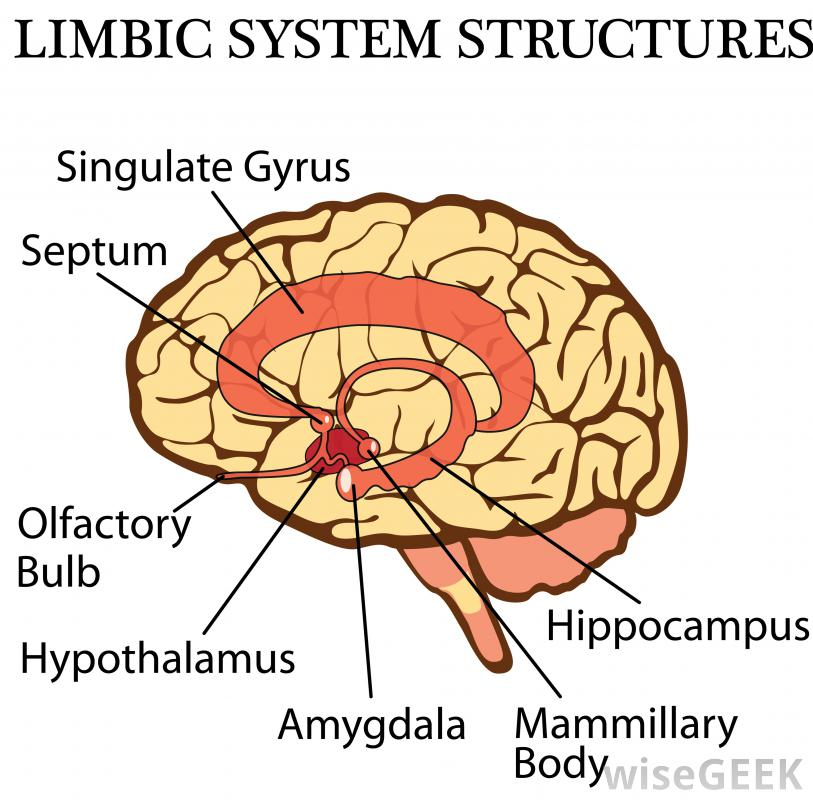
\includegraphics[width=6cm]{images/limbicsystem.jpg}
\caption{Limbic System}
\label{fig: Limbic System}
\end{figure}

More aromas: 
\begin{itemize}
    \item Durian
        \subitem Alfred Russel Wallace (1823-1913) the great naturalist had very praising comments for the fruit
        \subitem Aromatic essence of durian is a mixture of numerous chemicals: Propanethiol (oniony aroma) and methylbutyrate (pineappley aroma) most significant. 
        \subitem Smelly molecules include thiols and other sulfer compounds, esters, and ketones    
    \item Truffle Mushrooms
        \subitem White truffle (Tuber magnatum) and black truffle (Tuber melanosporum)
        \subitem Aromic qualities incredible
        \subitem Key component 2,4-dithiapentane
\end{itemize}

\subsection{Pheromones}

\textbf{Pheromones:} Chemicals that carry signal information related to social communications between members of the same species. \\
Play important roles in identity and social status, mate attraction, territorial and trail marking, and signaling of danger. \\

\noindent \textbf{Vomeronasal system:} distinct olfactory sensory structure and neural pathway that responds somewhat selectively to pheromone molecules. \\
However, some pheromones detected by receptors in main olfactory pathway. Highly debated whether this system has any effects in humans. \\

"Smell is primal. We haven't forgotten it. And it hasn't forgotten us." -Presti

% Olfactory epithelium, cilia \\
% Olfactory receptor cells, nasal ipthelium structural cells, mucus layer \\
% Olfactory stem cells, Olfactory nerve fibers to brain \\

% Stem cells because we are constantly exposed to toxic chemicals in our world, so it would be best if our cells are fresh to react accordingly \\
% Olfactory receptor proteins are GPCRs \\
% Mice 1300 functional olfactory receptors \\
% Humans 350 functional olfactory receptors, 100,000 diff odors \\

% cinnamon got some molecular components my dude \\
% cardomom my dude \\
% saffron \\
% black pepper \\
% rose \\
% jasmine, benzyl acetate \\
% perfumery: natural products vs. synthetic \\
% asparagus smell in urine, methanethiol, dimethylsulfide \\
% anomsmia, specifi anosmias \\



\end{document}
